% The underlying theory of the report

\subsection{One digital pixel}\label{sec:oneDigitalPixel}


Each pixel in the camera is constructed as shown in figure~\ref{fig:pixelschematic}.
The photo diodes detecting the actual light does, in many ways, act as a current source dependent on the light on it. When a picture is taken this
current is let through the transistor M1 and used to charge the capacitor CS. This is effectively converting a current-driven signal into a voltage level, to take into account the effects we get by exposing over time.
Before each picture is taken, the transistor M2 is opened to reset the voltage stored over CS.

It is important that M1 and M2 are not let on simultaneously for extended periods of time as this results in a short circuit from VDD to VSS through the photo diode PD1.
While the photo diode limits the current, this still might lead to excessive power usage and subsequent heating issues over time.

Another important value is the value for the capacitance of CS, which needs to be scaled in such a way that we get the maximum dynamic range for the pixel given the exposure times of the camera. The stored current in the capacitor needs to reach peak or convergence exactly when the camera reaches maximum exposure time with maximum brightness on the photo diode.


\begin{figure}[htbp]
  \centering
  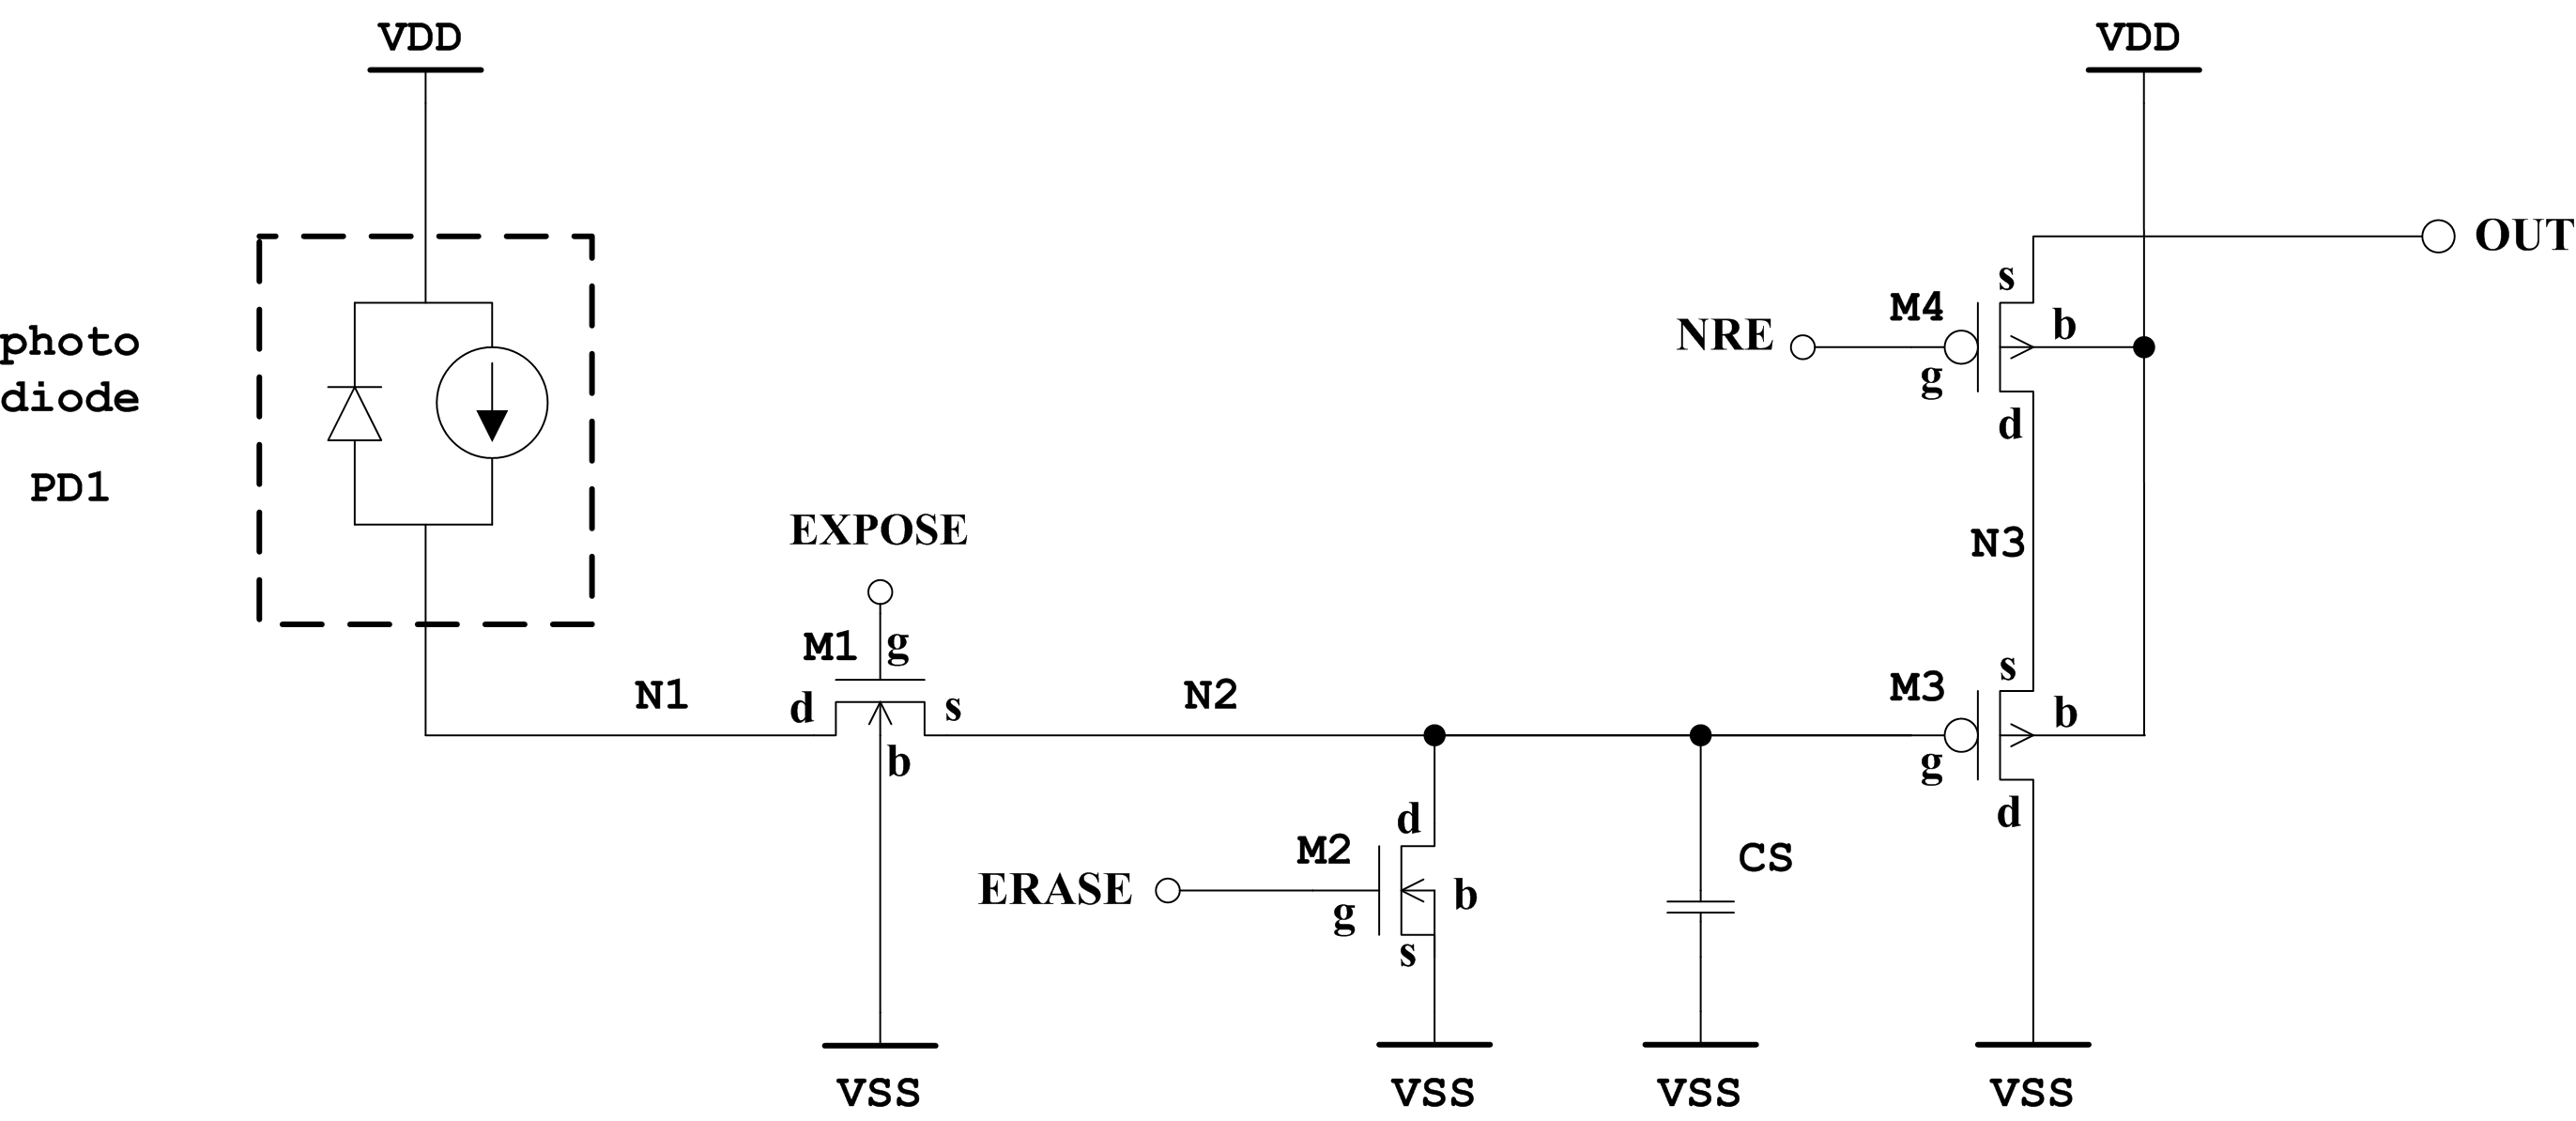
\includegraphics[width=0.80\textwidth]{figures/pixel}
  \caption{Schematic of one pixel with readout circuit, figure from~\cite{oppgave}}\label{fig:pixelschematic}
\end{figure}


The transistor M3 is used to convert the voltage stored over CS into a variable resistance between the nodes N3 and VSS for a nondestructive readout of the pixel. M1 should be closed whenever a picture is not being currently taken. The transistor M4 functions as a simple switch to isolate the pixel from OUT to free the wire when other pixels in the camera are using it.


\subsection{Leakage through transistors}\label{sec:leakagecurrent}

In this project we will assume that all voltage transient are so slow that no leakage current is present between gate and the other ports of any of the transistors,
in the same way we assume there is no leakage currents through any of the capacitors.

As described in Analog~integrated~circuit~design~\cite{AnalogBook} the current from drain to source $I_D \propto \frac{W}{L}$.
This also makes sense from a geometric point of view.

In order to minimize the leakage current through a transistor that is shut off $\frac{W}{L}$ should be minimized. The transistors are therefore optimized with this in mind, this is especially important for M2, which cannot let the capacitor drain while not being erased intentionally.


\subsection{Conceptual workings of a camera controller}

As shown in figure~\ref{fig:analogCamera} found in Appendix~\ref{ap:Schematics}, the behaviour of the pixels depend on several digital input signals,
the job of the camera controller is therefore to trigger these in the desired order.
The requirements to be met by the controller are the following:

\begin{itemize}
\item Pull the erase pin high except when exposing or reading the image
\item Pull the expose pin high for an appropriate length of time as defined by the user
\item Read out the values of all pixels in the correct order avoiding interference between different pixels connected to the same ADC.
\item Enable the user to reset the whole system at any time. Though the image being taken might be lost the camera should function normally afterwards.
\end{itemize}
